\begin{frame}{The Data Matrix}
    %Observations, variables, data matrices
    \begin{center}
        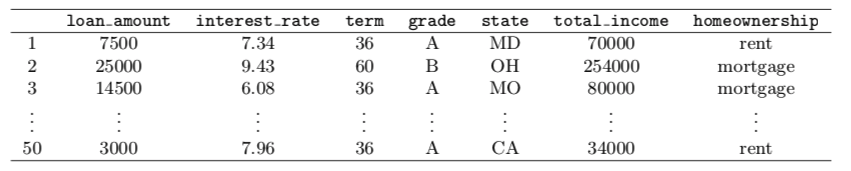
\includegraphics[scale=0.4]{datamatrix.png}
    \end{center}
    This \textbf{data matrix} shows rows 1, 2, 3, and 50 of a data set on loans. 
    \begin{itemize}
        \item Each row represents one loan.
        \item We call each row a \textbf{case} or \textbf{observational unit}. We \textit{observe} a number of different characteristics on each \textit{unit}.
        \item Each column represents some measured characteristic.
        \item We call these characteristics \textbf{variables} because they can \textit{vary} between observations. 
    \end{itemize}
\end{frame}

\begin{frame}{Understanding Our Data}
    \begin{center}
        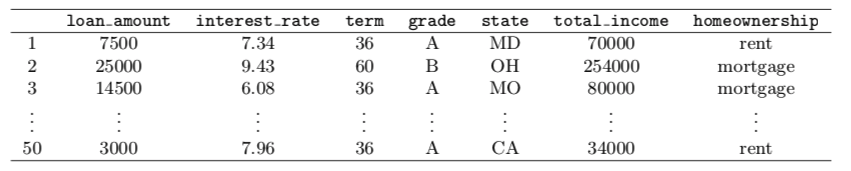
\includegraphics[scale=0.4]{datamatrix.png}
    \end{center}
    Whenever, we have data, it's important to start by making sure that we understand it. 
    \begin{itemize}
        \item What are some questions we might want to ask ourselves about this data set?
    \end{itemize}
\end{frame}

\begin{frame}{Understanding Our Data}
    Here are a few things I like to consider for all data sets:
    \begin{itemize}
        \item What does each variable represent?
        \item What are the units?
        \item Does the data make sense?
        \begin{itemize}
            \item What if the data showed an interest rate of $-999$?
            \item ...or a state labelled "42"?
        \end{itemize}
    \end{itemize}
\end{frame}

\begin{frame}{Types of Variables}
    Let's return to our data set:
    \begin{center}
        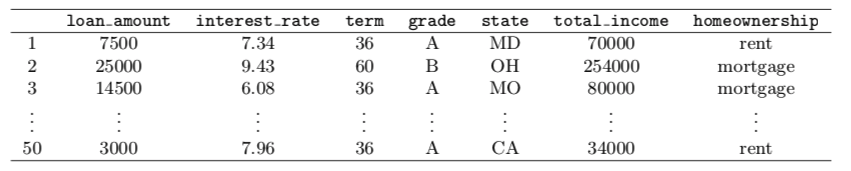
\includegraphics[scale=0.4]{datamatrix.png}
    \end{center}
    Notice that we have some variables made up of letters and some of numbers. This is the basic concept behind variable types. 
\end{frame}

\begin{frame}{Types of Variables}
    \begin{itemize}
        \item \textbf{Categorical}
        \begin{itemize}
            \item The responses are \textit{categories}.
            \item The state variable in our data set can take one of 50 possible values. 
        \end{itemize}
        \item \textbf{Numeric}
        \begin{itemize}
            \item The responses are \textit{numeric}.
            \item The numbers are meaningful (it makes sense to add, subtract, or take an average using those values). 
        \end{itemize}
    \end{itemize}
\end{frame}

\begin{frame}{Types of Numeric Variables}
    \begin{itemize}
        \item \textbf{Discrete}
        \begin{itemize}
            \item The responses can take on only whole number values.
            \item Population count is a discrete variable.
        \end{itemize}
        \item \textbf{Continuous}
        \begin{itemize}
            \item The responses can take on values on a continuous scale - there is no jump from one value to the next.
            \item Unemployment rate is a continuous variable. 
        \end{itemize}
    \end{itemize}
\end{frame}

\begin{frame}{Types of Variables}
    \begin{center}
        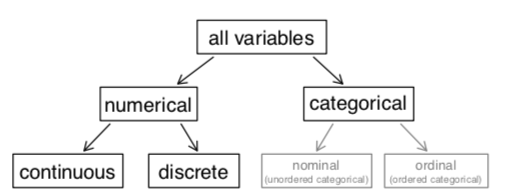
\includegraphics[scale=0.5]{vartypes.png}
    \end{center}
    Note: there are also two types of categorical variables.
    \begin{itemize}
        \item Ordinal variables are ordered (e.g., "like", "neutral", "dislike").
        \item Nominal variables are unordered (e.g., US states).
    \end{itemize}
\end{frame}

\begin{frame}{Relationships Between Variables}
    Our brains are constantly working on relationships between variables!
    \begin{itemize}
        \item Imagine if you walked down a flight of stairs outside your apartment 10 times and 9 of those times you fell down the stairs.
        \item You'd probably decide that something needs to change! Maybe you need to add some traction... or you need an extra cup of coffee before heading out in the morning. 
        \item In statistical terms, you decided that walking down those particular stairs relates to your falling down. You then make adjustments based on that association. 
    \end{itemize}
\end{frame}

\begin{frame}{Relationships Between Variables}
    Statistics takes these kinds of questions about how variables relate to one another (if I go out today, how likely am I to fall down the stairs?) and formalizes them so that we can make sound scientific claims.
\end{frame}

\begin{frame}{Relationships Between Variables}
    We can start thinking about how variables relate to one another through data visualization. 
    
    \begin{center}
        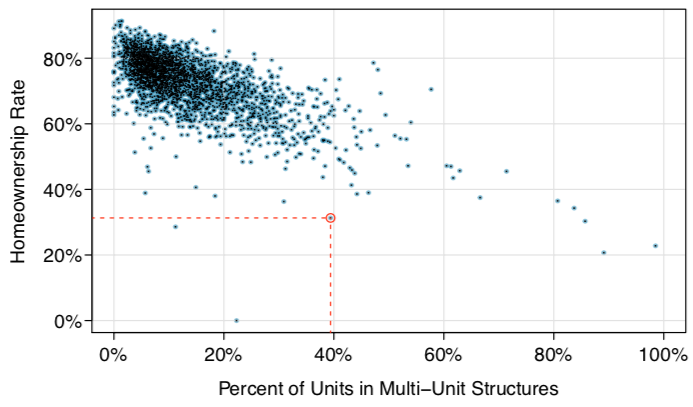
\includegraphics[scale=0.3]{scatter.png}
    \end{center}
    
    \vspace{-0.4cm}
    Consider the \textbf{scatterplot}. Do you think there's a relationship between a county's home ownership rate and its percent of units in multi-unit structures? Why might that be?
\end{frame}

\begin{frame}{Relationships Between Variables}
    \begin{center}
        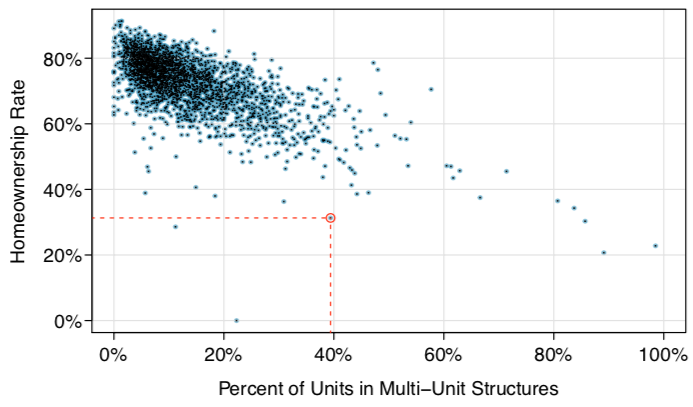
\includegraphics[scale=0.25]{scatter.png}
    \end{center}
    
    There is a clear pattern in the plot, so we say that these two variables are \textbf{associated}.
    \begin{itemize}
        \item Associated variables \textit{depend} on each other, so we say that they are \textbf{dependent variables}. 
        \item If two variables are not associated (no pattern), we say that they are \textbf{independent variables}.
    \end{itemize}
\end{frame}

\begin{frame}{Trend}
    \begin{center}
        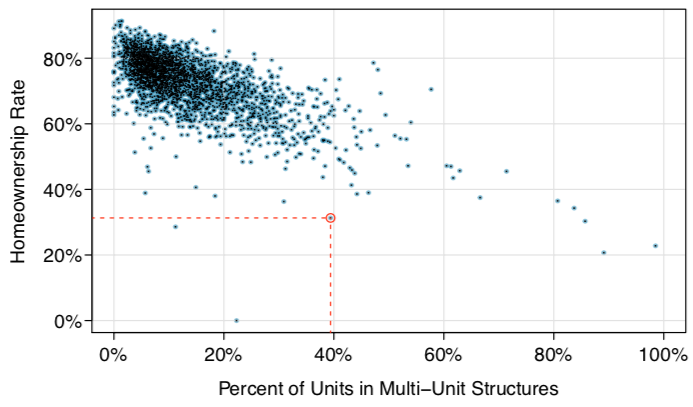
\includegraphics[scale=0.25]{scatter.png}
    \end{center}
    
    When two variables are related, we can consider the \textbf{trend}. 
    \begin{itemize}
        \item Here, there is a downward trend, suggesting that these two variables are \textbf{negatively associated}. 
        \item When we see an upward trend, we say that the variables are \textbf{positively associated}.
    \end{itemize}
\end{frame}

\begin{frame}{A Note on Correlation vs Causation}
    Who has heard someone say that "correlation is not causation"? 
    
    \vspace{1cm}
    Can you think of an example of two things that correlate but neither one causes the other?
\end{frame}

\begin{frame}{Correlation vs Causation}
    \begin{center}
        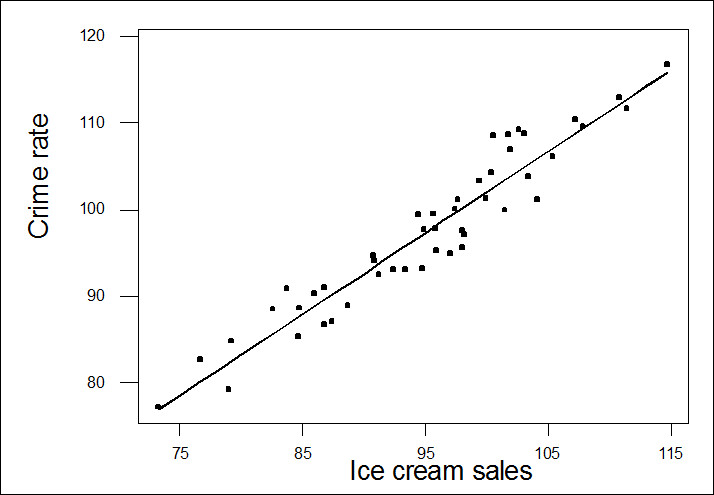
\includegraphics[scale=0.9]{icecream.jpeg}
    \end{center}
\end{frame}

\begin{frame}{Explanatory and Response Variables}
    Sometimes we do have causal questions. For example, suppose we have the following question:
    
    \begin{center}
        \textit{If there is an increase in the median household income in a county, does this drive an increase in its population?}
    \end{center}
    
    \begin{itemize}
        \item Median household income is an \textbf{explanatory variable}.
        \begin{itemize}
            \item We want to know if increases in median household income \textit{explain} population increases.
        \end{itemize}
        \item Population increase is a \textbf{response variable}.
        \begin{itemize}
            \item We want to know if the population increases \textit{in response to} increased median household income. 
        \end{itemize}
    \end{itemize} 
\end{frame}

\begin{frame}{Explanatory and Response Variables}
    When we predict some causal relationship, we can label our variables accordingly.
    
    \begin{center}
        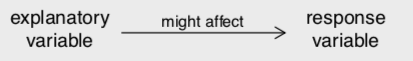
\includegraphics[scale=0.5]{affect.png}
    \end{center} 
    
    However, predicting causality and labeling variables as explanatory and response does \textit{not} guarantee that a causal relationship actually exists. 
    
    \vspace{12pt}
    (Remember our ice cream example - we can be wrong in our predictions but still find an association! )

\end{frame}